\documentclass{scrartcl}
% \usepackage{hyperref}
% \usepackage{tikz}
\usepackage{amsmath}
\usepackage{amsthm}
\usepackage{pifont}
\usepackage{mathrsfs}
\usepackage{amssymb}
\usepackage{xcolor}
\usepackage{colortbl}
\usepackage{tikz-cd}
\usepackage{caption}
\usepackage{newunicodechar}


\usepackage[utf8]{inputenc}
\usepackage{ucs}
% \DeclareUnicodeCharacter{03A3}{\ensuremath{\Sigma}}



\usetikzlibrary{positioning,shapes.geometric,fit,arrows.meta}


\captionsetup{justification=centering}


\usepackage{hyperref}
% \usepackage{tikz}
\usepackage{amsmath}
\usepackage{amsthm}
\usepackage{pifont}
\usepackage{mathrsfs}
\usepackage{amssymb}
\usepackage{xcolor}
\usepackage{colortbl}
\usepackage{tikz-cd}
\usepackage{caption}
\usepackage{newunicodechar}


\usepackage[utf8]{inputenc}
\usepackage{ucs}
% \DeclareUnicodeCharacter{03A3}{\ensuremath{\Sigma}}



\usetikzlibrary{positioning,shapes.geometric,fit,arrows.meta}


\captionsetup{justification=centering}



\definecolor{darkgreen}{rgb}{0.0, 0.5, 0.0}

\newcommand{\tto}{\twoheadrightarrow}
\newcommand{\sse}{\subseteq}
\newcommand{\bset}{\mathbf{Set}}
\newcommand{\nat}{\mathbb{N}}

% Comments
\newcommand{\sacomment}[1]{\textcolor{green}{#1}}
\newcommand{\apcomment}[1]{\textcolor{blue}{#1}}
\newcommand{\greyout}[1]{\textcolor{gray}{#1}}
\newcommand{\err}[1]{\textcolor{red}{#1}}

% Theorem style
% \newtheorem{thm}{Theorem}
% \newtheorem{dfn}[thm]{Definition}
% \newtheorem{prop}[thm]{Proposition}
% \newtheorem{cor}[thm]{Corollary}
% % \newtheorem{lemma}[thm]{Lemma}
% % \newtheorem{rmk}[thm]{Remark}
% % \newtheorem{expl}[thm]{Example}
% \newtheorem{notn}[thm]{Notation}
% %\theoremstyle{nonumberplain}
% %\theoremsymbol{\Box}
% % \newtheorem{proof}{Proof}

\newcommand{\RP}{\mathrm{RP}}
\newcommand{\gRP}{\mathbf{RP}}
\newcommand{\RPm}{\mathrm{RP^{-}}}
\newcommand{\gRPm}{\mathbf{RP^{-}}}
\newcommand{\NF}{\mathrm{NF}}
\newcommand{\MF}{\mathrm{MF}}
\newcommand{\UN}{\mathrm{UN}}
\newcommand{\gUN}{\mathbf{UN}}
\newcommand{\UNto}{\mathrm{UN}^{\to}}
\newcommand{\gUNto}{\mathbf{UN}^{\to}}
\newcommand{\SN}{\mathrm{SN}}
\newcommand{\gSN}{\mathbf{SN}}
\newcommand{\decSN}{\mathrm{dec(SN)}}
\newcommand{\SM}{\mathrm{SM}}
\newcommand{\SMseq}{\mathrm{SMseq}}
\newcommand{\gSMseq}{\mathbf{SMseq}}
\newcommand{\gSM}{\mathbf{SM}}
\newcommand{\WN}{\mathrm{WN}}
\newcommand{\gWN}{\mathbf{WN}}
\newcommand{\SMandWN}{\mathrm{SM\land WN}}
\newcommand{\gSMandWN}{\mathbf{SM\land WN}}
\newcommand{\WM}{\mathrm{WM}}
\newcommand{\gWM}{\mathbf{WM}}
\newcommand{\WNFP}{\mathrm{WNFP}}
\newcommand{\NP}{\mathrm{NP}}
\newcommand{\gNP}{\mathbf{NP}}
\newcommand{\NPe}{\mathrm{NP_=}}
\newcommand{\gNPe}{\mathbf{NP_=}}
\newcommand{\WMFP}{\mathrm{WMFP}}
\newcommand{\MP}{\mathrm{MP}}
\newcommand{\gMP}{\mathbf{MP}}
\newcommand{\CR}{\mathrm{CR}}
\newcommand{\CRs}{\mathrm{CR^{\le 1}}}
\newcommand{\gCRs}{\mathbf{CR^{\le 1}}}
\newcommand{\gCR}{\mathbf{CR}}
\newcommand{\WCR}{\mathrm{WCR}}
\newcommand{\gWCR}{\mathbf{WCR}}
\newcommand{\Inc}{\mathrm{Inc}}
\newcommand{\gInc}{\mathbf{Inc}}
% \newcommand{\BP}{\mathrm{BP}}
\newcommand{\gBP}{\mathbf{BP}}
\newcommand{\FB}{\mathrm{FB}}
\newcommand{\CP}{\mathrm{CP}}
\newcommand{\gCP}{\mathbf{CP}}



\newcommand{\from}{\leftarrow}



\newcommand{\red}[1]{\textcolor{red}{#1}}
\newcommand{\blue}[1]{\textcolor{blue}{#1}}

% Reduction relation macros
\newcommand{\rstep}{\mathbin{\longrightarrow_R}}
\newcommand{\mstep}{\mathbin{\longrightarrow_R^*}}
\newcommand{\estep}{\mathbin{\longrightarrow_R^=}}
\newcommand{\rrstep}{\mathbin{\longrightarrow_R^r}}
\newcommand{\brstep}{\mathbin{\longleftarrow_R^r}}
\newcommand{\bstep}{\mathbin{\longleftarrow_R}}
\newcommand{\bmstep}{\mathbin{\longleftarrow_R^*}}

% Unicode characters

\newunicodechar{∀}{\ensuremath{\forall}}
\newunicodechar{→}{\ensuremath{\rightarrow}}
\newunicodechar{ℕ}{\ensuremath{\mathbb{N}}}
\newunicodechar{↔}{\ensuremath{\leftrightarrow}}
\newunicodechar{⊆}{\ensuremath{\sse}}
\newunicodechar{∧}{\ensuremath{\land}}
\newunicodechar{₌}{\ensuremath{_=}}
\newunicodechar{𝓟}{\ensuremath{\mathcal{P}}}
\newunicodechar{∈}{\ensuremath{\in}}
\newunicodechar{φ}{\ensuremath{\phi}}
\newunicodechar{Σ}{\ensuremath{\Sigma}}
\newunicodechar{₁}{\ensuremath{{}_1}}


% Misc Macros
\newcommand{\terese}{[TeReSe]}
% \newcommand{\ul}[1]{\underline{#1}}
\newcommand{\ule}[1]{\underline{#1:}}
% \newcommand{\setof}[1]{\{#1\}}
\newcommand{\setof}[1]{\left\{#1\right\}}


\newcommand{\tclos}[1]{{#1}^{\scriptscriptstyle{+}}}


% Taken from well founded section

\newcommand{\isWFacc}{\mathtt{isWFacc}}
\newcommand{\isWFseq}{\mathtt{isWFseq}}
\newcommand{\isWFmin}{\mathtt{isWFmin}}
\newcommand{\isWFaccm}{\mathtt{isWFacc-}}
\newcommand{\isWFseqm}{\mathtt{isWFseq-}}
\newcommand{\isWFminm}{\mathtt{isWFmin-}}

\newcommand{\isMinDec}{\mathtt{isMinDec}}


\title{Summer 2024 Report}
\author{Sam Arkle}
\date{\today}

\begin{document}

\maketitle

\tableofcontents

\section{Introduction}
This is a report on the progress I have made during the summer of 2024 working with Dr. Polonsky \footnote{Assisstant Professor, Department of Computer Science, Appalachian State University.}. I have been writing on the topic of relations, working primarily from Term Rewriting Systems (TeReSe) \footnote{(Term Rewriting Systems. (2003). United Kingdom: Cambridge University Press.)}.
The objective of this work has been to both develop a formal understanding of relations and to build a library in Agda \footnote{\href{https://github.com/DrPolonsky/LAM/tree/main/Relations}{Github repository for this project's code}} that will be used as a foundation to further work in theoretical computer science.
\\
I have been focussed on Chapter 1 of TeReSe which covers abstract reduction systems (ARS) as well as the appendix (sections 1-3) which provides the necessary mathematical background for the rest of the book (e.g. relations, ordinals, inductive definitions and the Knaster-Tarski lemma). Where the book has made use of classical logic I have investigated the possibility of using constructive alternatives.

\section{Definitions}
The most interesting work we have carried out in investigating Chapter 1 of TeReSe has resulted from trying to provide constructive proofs for Newman's lemma, the Knaster-Tarski lemma, theorem 1.2.2 and theorem 1.2.3. Before exploring those proofs the following definitions are essential.


The following definitions are taken from [TeReSe], Chapter 1,
with minimal adaptations for consistency.

\begin{dfn}
  An abstract reduction system (\emph{ARS}) is a structure $\mathcal{A} = (A, R_\alpha)$ where $A$ is a set and $R_\alpha$ is a set of binary relations.
\end{dfn}
A relation $R$ from the set $R_\alpha$ is refered to as a reduction (or rewrite) relation. For example, if we specify $R$ as the relation of being 'less than' ($<$) then $R\, 4\, 2$. \textcolor{red}{Right?}
\apcomment{Yes, but move this to a(n eventual) list of examples.}

We use $R$ or $\to$ for a single-step reduction and $R^*$ or $\tto$ for a multi-step reduction.

\sacomment{Should we be using $R^+$ rather than $R^*$?}

\apcomment{Thus, when $(a,b) \in \to_{(\alpha)}$, we say that there is a
\emph{$(\alpha-)$reduction} from $a$ to $b$.
When $(a,b) \in \tto_\alpha$, we say that there is a multi-step $\alpha$-reduction
from $a$ to $b$.}

\begin{dfn}
  An element $a \in A$ is \emph{R-weakly confluent} ($WCR_R$) if all single step reductions from $a$ can always converge
  via multi-step reductions to some common reduct.
  A relation $R$ is \emph{weakly confluent} (AKA weakly Church-Rosser (WCR)) if every $a \in A$ is R-weakly confluent.
\end{dfn}

\begin{dfn}
  An element $a \in A$ is \emph{R-confluent} ($CR_R$) if all multi-step reductions from $a$ can always converge
  via multi-step reductions to some common reduct.
  A relation $R$ is \emph{confluent} (AKA Church-Rosser (CR)) if every $a \in A$ is R-confluent.
\end{dfn}

\begin{figure}[h]
  \centering
\[  \begin{tikzpicture}[node distance=1.5cm, auto]
    % Nodes
    \node (top) {a};
    \node (left) [below left of=top] {b};
    \node (right) [below right of=top] {c};
    \node (bottom) [below right of=left] {d};

    % Arrows
    \draw[->] (top) -- (left);
    \draw[->] (top) -- (right);
    \draw[->>] (left) -- (bottom);
    \draw[->>] (right) -- (bottom);
\end{tikzpicture}
\hspace{3cm}
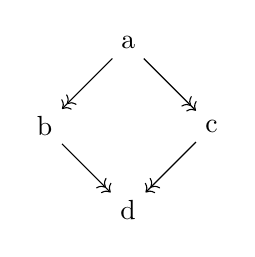
\begin{tikzpicture}[node distance=1.5cm, auto]
  % Nodes
  \node (top) {a};
  \node (left) [below left of=top] {b};
  \node (right) [below right of=top] {c};
  \node (bottom) [below right of=left] {d};

  % Arrows
  \draw[->>] (top) -- (left);
  \draw[->>] (top) -- (right);
  \draw[->>] (left) -- (bottom);
  \draw[->>] (right) -- (bottom);
\end{tikzpicture}
\]
\caption{On the left is an example of a weakly confluent relation. On the right is an example of a confluent relation.}
\end{figure}


\begin{dfn}
  \emph An element $a \in A$ is a {normal form} if there exists no reduction to any other element in $A$.
\end{dfn}

\begin{dfn}
  An element $a \in A$ is \emph{$R$-weakly normalizing} ($WN_{R}$)if $a \tto b$ for some normal form $b \in A$.

  A relation $R$ is weakly normalizing (WN) if every $a \in A$ is $R$- weakly normalizing.
\end{dfn}

\begin{dfn}
  An element $a \in A$ is \emph{$R$-strongly normalizing} ($SN_R$) if every reduction sequence starting from $a$ is finite.

  A relation $R$ is strongly normalizing (SN) if every
  $a \in A$ is $R$-strongly normalizing.
\end{dfn}

The above definition of SN is taken from [TeReSe]. When working in Agda, we make use of the alternative definition presented in [TeReSe] ($\leftarrow$ is accessibly well-founded).

\subsection{Closure operations on relations}

A relation $R$ has the following properties when the stated conditions are met:
\begin{dfn}
  \emph{reflexive} {- $\forall x \in A : x \to x $}
\end{dfn}
\begin{dfn}
  \emph{transitive} {- $\forall x, y, z \in A : ( x \to y \land y \to z ) \implies x \to z $}
\end{dfn}
\begin{dfn}
  \emph{symmetric} {- $\forall x, y \in A : x \to y \implies y \to x$}
\end{dfn}

\begin{dfn}
  The \emph{closure} of $R$ is the smallest relation that contains $\to$ and satisfies a given property.
\end{dfn}

\begin{dfn}
  The \emph{reflexive closure} of $R$ is the smallest relation $\to^r$ that contains $\to$ and is reflexive.
\end{dfn}
\begin{dfn}
  The \emph{symmetric closure} of $R$ is the smallest relation $R^s$ that contains $R$ and is symmetric.
\end{dfn}
\begin{dfn}
  The \emph{transitive closure} of $R$ is the smallest relation $R^+$ that contains $R$ and is transitive.
\end{dfn}
\begin{dfn}
  The \emph{reflexive transitive closure} of $R$ is the smallest relation $R^*$ that contains $R$ and is both reflexive and transitive.
\end{dfn}
\begin{dfn}
  The \emph{equivalence relation} of $R$ is the smallest relation $R^=$ that contains $R$ and is reflexive, transitive, and symmetric.
\end{dfn}

\begin{dfn}
  A relation $R$ has the \emph{normal form property} (NFP) if
 $a \to^= b$  $\implies$
 $a \tto b$, for all $a \in A$ and any normal form $b \in A$.
\end{dfn}

Two elements $a, b \in A$ being equivalent is denoted $a \equiv b$.

\begin{dfn}
  A relation $R$ has the \emph{unique normal form property} (UN) if
  $a \to^= b$  $\implies$
  $a \equiv b$, for all $a \in A$ and any normal form $b \in A$.
\end{dfn}

\begin{dfn}
  A relation $R$ has the \emph{unique normal form property with respect to reduction} (UN$^ \to$) if
  $a \twoheadleftarrow  \cdot  \tto b$  $\implies$ $a \equiv b$, for all normal forms $a,b \in A$.
\end{dfn}

Let $A$ be a set.
\begin{dfn}
  A \emph{sequence (in $A$)} is a function from the natural numbers to $A$:
  \begin{align*}
    &s : \nat \to A \\
    &s = (s_0,s_1,s_2,\dots)
  \end{align*}
\end{dfn}

\begin{dfn}
  A sequence is \emph{$R$-increasing} if every term is $R$-related to its preceding term.
\end{dfn}

\begin{dfn}
  A sequence is \emph{bounded} if there exists an element $a$ to which all elements of the sequence reduce.
\end{dfn}

\begin{figure}[h]
  \centering
  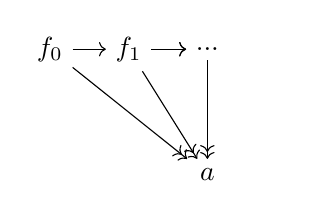
\begin{tikzpicture}
      % Define the nodes inside the region f
      \node (f0) at (0, 0) {$f_0$};
      \node (f1) at (1, 0) {$f_1$};
      \node (dots) at (2, 0) {$...$};

      % Draw the arrows between the nodes inside the region f
      \draw[->] (f0) -- (f1);
      \draw[->] (f1) -- (dots);
      \draw[->] (f1) -- (dots);


      % Define the nodes outside the region f
      \node (a) [below=of dots, yshift=-.25cm] {\parbox{2cm}{\centering $a$ }};

          % Draw the arrows between the nodes inside and outside the region f sds

          \draw[->>] (f0) -- (a);
          \draw[->>] (f1) -- (a);
          \draw[->>] (dots) -- (a);
      \end{tikzpicture}
      \caption{An example of an bounded sequence.}

    \end{figure}


\begin{dfn}
  An element $a \in A$ has the \emph{recurrence property} if $a \tto b \implies b \tto a$ for all $b \in A$.
\end{dfn}
\sacomment{I've been using $\tto$ as interchangable with $R *$ (as in the above definition).
Is that okay or am I going to have to clarify why they are interchangable (are they not interchangable?)?}
\apcomment{It's okay, but later we will need to make sure we are using them consistently.  Say that in Agda code, $\to$ is denoted by $R$.}

\begin{dfn}
  A relation $R$ has the \emph{recurrence property} (RP) if every
  bounded, increasing sequence has a recurrent element.
\end{dfn}

    \begin{figure}[h]
      \centering
      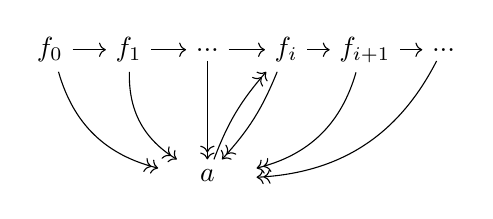
\begin{tikzpicture}
          % Define the nodes inside the region f
          \node (f0) at (0, 0) {$f_0$};
          \node (f1) at (1, 0) {$f_1$};
          \node (dots) at (2, 0) {$...$};
          \node (fi) at (3, 0) {$f_i$};
          \node (fi+1) at (4, 0) {$f_{i+1}$};
          \node (dots2) at (5,0) {$...$};

          % Draw the arrows between the nodes inside the region f
          \draw[->] (f0) -- (f1);
          \draw[->] (f1) -- (dots);
          \draw[->] (dots) -- (fi);
          \draw[->] (fi) -- (fi+1);
          \draw[->] (fi+1) -- (dots2);


          % Define the nodes outside the region f
          \node (a) [below=of dots, yshift=-.25cm] {\parbox{1cm}{\centering $a$ }};

              % Draw the arrows between the nodes inside and outside the region f sds

              \draw[->>] (f0) to [bend right] (a);
              \draw[->>] (f1) to [bend right] (a);
              \draw[->>] (dots) -- (a);
              \draw[->>] (fi) to [bend left=10] (a);
              \draw[->>] (fi+1) to [bend left] (a);
              \draw[->>] (dots2) to [bend left] (a);
              \draw[->>] (a) to [bend left=10] (fi);

          \end{tikzpicture}
          \caption{An example of a relation with the recurrence property.}

        \end{figure}
\begin{dfn}
  A relation $R$ has the \emph{weak recurrence property} (RP-) if
  for every increasing sequence with bound $a$,
  there is an element $i$ of the sequence such that $a \tto f (i)$.
\end{dfn}


\begin{dfn}
  \emph{Cofinality property}
\end{dfn}
\sacomment{Still not sure on how to define cofinality.}

\begin{dfn}
  A relation $R$ is \emph{finitely branching} (FB) if, for all $a \in A$, the set of one step reducts of $a$ is finite.
\end{dfn}

\subsection{Recurrence property and increasing relations}

In [TeReSe], a relation $R \sse A \times A$ is called \emph{increasing} if there
exists a ``size function'' $|-| : A \to \nat$ satisfying, for all $x, y \in A$,
 \[ Rxy \to |x| < |y| \]

\begin{prop}
  If $R$ is increasing, then no infinite $R$-increasing sequence is bounded.
\end{prop}
\begin{proof}
  Let $(a_i) = a_0 \to a_1 \to a_2 \to \cdots$ be an $R$-increasing sequence
  and suppose that $(a_i)$ is bounded.  Let $b$ be the bound, so that $a_i \to b$ for all $i$.

  If $m = |b|$ then we have
  \[ 0 \le |a_0| < |a_1| < |a_2| < \cdots < |a_m| < |b| = m \]
  % \[ m > |a_m| > |a_{m-1}| > \cdots > |a_0| \ge 0 \]
  which is a contradiction, since there are only $m-1$ integers strictly less than $m$.
\end{proof}

It follows that every relation that is increasing in the sense of [TeReSe]
vacuously satisfies the RP condition.

\begin{cor}
  If $R$ is increasing, then $R$ has the recurrence property.
\end{cor}


\section{Classical Principles}
Principles we are considering
\begin{itemize}
  \item Decidability of equality on $A$
  \item Decidability of the relation $R$
  \item When relevant, decidability of the given precicate $P$
  \item Not-not-closure of being accessible
  \item Not-not-closure of $R$
  \item Not-not-closure of $P$
  \item Decidability of whether a given element is an $R$-normal form
  \item When relevant, local/element-wise versions of the above
  \item Markov's principle:
  \begin{itemize}
    \item In $wfMin_0 \to wfSeq$.

    Given a sequence $s : \nat \to A$, let $E(a) = \exists n \in \nat. s n \equiv a$.

    Need: $\forall a. \lnot\lnot E(a) \to E(a)$, i.e.,
    \[\lnot\lnot \big(\exists n \in \nat. s n \equiv a\big)
          \to \big(\exists n \in \nat. s n \equiv a\big)\]

  \end{itemize}
\end{itemize}

\section{Implications}
We now look into the interrelation of the various properties defined in Section 2. Our aim is to expand on the
connections made in Figure 1.8 of [TeReSe] (p.19).

\section{Counterexamples}
The following counterexamples are used to rule out certain implications between properties from holding.
\sacomment{How should we present this section. Is it enough to have diagrams and a list of what they are a counter to?}
\subsection*{Counterexample 1}
\begin{center}

  \begin{tikzcd}[node distance=2cm, auto]
      % Nodes
      \node (a) {a};
      \node (b) [right of=a, xshift=1cm] {b};
      \node (c) [right of=b, xshift=1cm] {c};
      \node (d) [right of=c, xshift=1cm] {d};

      % Arrows
      \draw[->] (b) to [bend left] (c);
      \draw[->] (c) to [bend left] (b);
      \draw[->] (b) -- (a);
      \draw[->] (c) -- (d);
  \end{tikzcd}

\end{center}
Counterexample to:
\begin{itemize}
  \item WCR $\implies$ CR
  \item WCR and WN $\implies$ CR
  \item WCR and WN $\implies$ SN
  \item \mbox{WCR R $\to$ $\forall$ a b $\to$ is R -NF b $\to$ (R *) a b $\to$ $\forall$ c $\to$ (R *) a c $\to$ (R *) c b}
  \item IOW and WCR $\implies$ WNFP \sacomment{We need to define these still (IOW and WNFP)}
\end{itemize}
\subsection*{Counterexample 2}
\begin{center}
  \begin{tikzcd}
      % Nodes
      \node (x) {x};
      \node (n) [left of=x, xshift=-1cm] {n \in NF};
      \node (y) [right of=x, xshift=1cm] {y};
      \node (z) [right of=y] {z};

      % Arrows
      \draw[->>] (x) -- (n);
      \draw[->>] (x) -- (y);
      \draw[->] (y) to [bend left] (z);
      \draw[->] (z) to [bend left] (y);
  \end{tikzcd}
\end{center}

Counterexample to:
\begin{itemize}
  \item WN$\downarrow\subseteq$WN (WN is not closed under reduction) \sacomment{Is this the right way to express that elementwise WN doesn't imply global WN?}
  \item WN$\downarrow$UN$\rightarrow\subseteq$WN :

  UN$\rightarrow\,$R $\to \forall$ x $\to$ is R-WN x $\to$ $\forall$ y $\to$ (R *) x y $\to$ is R-WN y

  \textcolor{red}{SA: The above is a bit messy, can we make it cleaner?}
  \item $\forall$ (R : $\mathscr{R}$ A) $\to$ $\forall$ is R -WN x $\to$ is R -UN x $\to$ is R -CR x
  \item $WN_R$ and $UN_R$ $\implies$ $CR_R$

\end{itemize}

\subsection*{Counterexample 3}

\begin{center}
  \begin{tikzcd}
      % Nodes
      \node (x) {x};

      % Arrows
      \draw[->, loop] (x) to (x);
  \end{tikzcd}
\end{center}
Counterexample to:
\begin{itemize}
  \item bounded and RP implies SN
  \item bounded and RP implies WN
\end{itemize}

\subsection*{Counterexample 4}
  \begin{center}
      \begin{tikzpicture}
      % Define the nodes
      \node (a) at (0, 0) {$a$};
      \node (b) at (1, 0) {$b$};
      \node (dots) at (2, 0) {$...$};

      % Draw the arrows
      \draw[->] (a) -- (b);
      \draw[->] (b) -- (dots);


      \end{tikzpicture}
    \end{center}
Counterexample to:


\section{Well-foundedness}
\subsection{Well-foundedness}
\sacomment{Talk about the different types of wellfoundedness, starting with the one given in the book, the reason for thinking it is classical and not constructive, and provide an image showing the relation between the notions of wellfoundedness we have. Talk about future work in this area.}

\apcomment{Mention that, for a set $A$, we will use "subset of $A$" and "predicate on $A$" interchangeably,
with subsets being represented in the Agda code using predicates, which are in turn formalized as
dependent types over $A$, i.e. maps $\phi : A \to \bset$ }

Working in constructive logic introduces subtle differences between notions of well-foundedness of relations
which are not present in classical logic.  In our investigation, we have focused on four distinct definitions of well-foundedness, with minor variations of each. To spell these out, we first define some preliminary notions.
% The make clear the difference between these distinct notions of well-foundedness we first present the following defintiions for a given relation $R$.

\begin{dfn} Let $A$ be a set and $R \sse A \times A$ be a relation.
\begin{enumerate}
  \item Let $\phi$ be a predicate on $A$. An element $x \in A$ is $R$-minimal for $\phi$ if $\phi(x)$ is true and no other element for which $\phi$ holds is $R$-related to $x$.
  \item An element $x \in A$ is \textit{$R$-accessible} if every element $R$-related to $x$ is \textit{$R$-accessible}.  (This should be understood as an inductive definition, with base case consisting of $R$-minimal elements for the whole of $A$.)
    \item A predicate $\phi$ on $A$ is \emph{inductive} if it holds on a given element $x \in A$ whenever it holds on all elements $R$-related to $x$:
    \[ (\forall y. Ryx \to \phi(y)) \to \phi(x) \]
    \item A sequence $s = (s_0,s_1,\dots)$ of elements of $A$ is $R$-decreasing
    if every element is related to its predecessor.  That is, $Rs_{n+1}s_n$ for all $n$.
\end{enumerate}
\end{dfn}
With the above definitions established we define the notions of well-foundedness we have been investigating.
\begin{dfn} \hfil
  \begin{enumerate}
    \item \textit{R} is well-founded if every element is \textit{R}-accessible.
    \item \textit{R} is well-founded if every inductive predicate is universally true.
    \item \textit{R} is well-founded if every non-empty predicate has a minimal element with respect to $R$.
    \item \textit{R} is well-founded if every sequence contains a non-decreasing index.
  \end{enumerate}
\end{dfn}
  Further, we explored weaker variants of these notions of well-foundedness.
  \begin{dfn} \hfil
    \begin{enumerate}
      \item \textit{R} is well-founded if every element is $\lnot \lnot$  \textit{R}-accessible.
      \item \textit{R} is well-founded if for every inductive predicate $\phi$, $\lnot \lnot \phi$ is universally true.
      \item \textit{R} is well-founded if it is not not the case that every non-empty predicate has a minimal element with respect to $R$. \textcolor{red}{is there a better way to express this double negation in english?}
      \item \textit{R} is well-founded if there is no infinite $R$-decreasing sequence (this is the definition of well-foundedness found in TeReSe).
    \end{enumerate}

\end{dfn}

\begin{figure}[h]
  \centering
  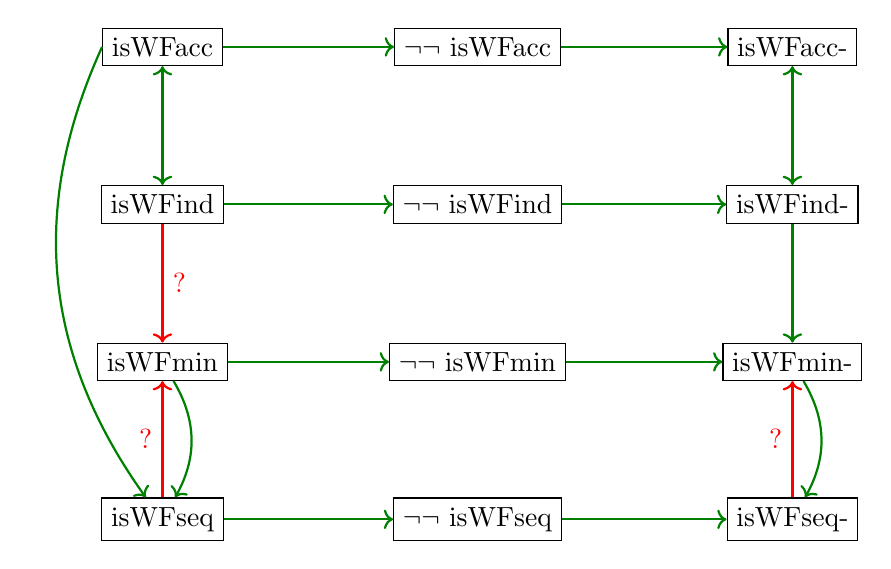
\begin{tikzpicture}[node distance=2cm, auto]
    % Standard definitions
    \node (std1) [draw] {isWFacc};
    \node (std2) [below of=std1, draw] {isWFind};
    \node (std3) [below of=std2, draw] {isWFmin};
    \node (std4) [below of=std3, draw] {isWFseq};

    % Double negation definitions
    \node (dn1) [right of=std1, xshift=2cm, draw] {$\lnot \lnot$ isWFacc};
    \node (dn2) [right of=std2, xshift=2cm, draw] {$\lnot \lnot$ isWFind};
    \node (dn3) [right of=std3, xshift=2cm, draw] {$\lnot \lnot$ isWFmin};
    \node (dn4) [right of=std4, xshift=2cm, draw] {$\lnot \lnot$ isWFseq};

    % Weaker definitions
    \node (weak1) [right of=dn1, xshift=2cm, draw] {isWFacc-};
    \node (weak2) [right of=dn2, xshift=2cm, draw] {isWFind-};
    \node (weak3) [right of=dn3, xshift=2cm, draw] {isWFmin-};
    \node (weak4) [right of=dn4, xshift=2cm, draw] {isWFseq-};

    % Arrows
    \draw[->, thick, darkgreen] (std1) -- (dn1);
    \draw[->, thick, darkgreen] (std1.west) to[out=180, in=90, bend right] (std4);
    \draw[->, thick, darkgreen] (dn1) -- (weak1);
    \draw[<->, thick, darkgreen] (std1) -- (std2);
    \draw[->, thick, darkgreen] (std2) -- (dn2);
    \draw[->, thick, darkgreen] (dn2) -- (weak2);
    \draw[<->, thick, darkgreen] (weak1) -- (weak2);
    \draw[->, thick, red] (std2) -- (std3) node[pos=0.5, right, red] {?};
    \draw[->, thick, darkgreen] (std3) -- (dn3);
    \draw[->, thick, darkgreen] (dn3) -- (weak3);
    \draw[->, thick, darkgreen] (weak2) -- (weak3);
    \draw[->, thick, darkgreen, bend left] (std3) to (std4);
    \draw[->, thick, darkgreen, bend left] (weak3) to (weak4);
    \draw[->, thick, darkgreen] (std4) -- (dn4);
    \draw[->, thick, darkgreen] (dn4) -- (weak4);
    \draw[->, thick, red, bend left] (std4) -- (std3) node[pos=0.5, left, red] {?};
    \draw[->, thick, red, bend left] (weak4) -- (weak3) node[pos=0.5, left, red] {?};
  \end{tikzpicture}
  \caption{A graphic illustrating the implications we have found between the above
  definitions and those we are still seeking to find. Green arrows indicate that one
  definition implies another, red arrows indicate that we believe an implication should
  be possible but we have not yet found it.
  }
\end{figure}



  As future work we want to know whether the missing implications can be found, or what the minimal additional requirements are for making those implications.

\section{Notes}
\subsection{Notes from 08.29}

\begin{enumerate}
  \item Try to ``fix'' CP by changing $R$ into $R^r$
  \item Finish formulating the ``compactness property".  Two candidates:
  \begin{itemize}
    \item ``Every cocone for a given infinite sequence loops back to some point in the sequence"
    \item ``If an $R^*$-sequence has a cocone then it's constant after some point on.''
  \end{itemize}
  \item Add the definition of "recurrent element"
\end{enumerate}

\subsection{09.05}
\begin{enumerate}
  \item done: WN, UN, RP imply SN (classical)
  \item need: omega bounded and RP implies SN (classical)
  \item need: omega bounded and RP implies SN (constructive)
  \item do we need $s_0 \to^* s_c$ in the proof?
  \item is $\omega$-bounded implied by WN and the following confluence property:
  $a \to^* n \in NF$, and $a \to b$ then $b \to^* n $.
  \item Remark before 1.2? (Exercise 1.3.21)
  \item Make the first argument to "being a normal form" implicit?
\end{enumerate}

\newcommand{\RP}{\mathsf{RP}}
\newcommand{\NF}{\mathsf{NF}}
\newcommand{\UN}{\mathsf{UN}}
\newcommand{\UNto}{\mathsf{UN}{\to}}
\newcommand{\SN}{\mathsf{SN}}
\newcommand{\WN}{\mathsf{WN}}
\newcommand{\from}{\leftarrow}

\subsection*{Additional remarks about Theorem 1.2.3.}
\begin{itemize}
  \item It seems that part (i) of the theorem can be strengthened to only
  assume $\UNto(R)$ instead of $\UN(R)$:
  \[ \WN(R) \land \UNto(R) \to \omega{-}\text{bounded}(R) \tag{i} \]
  \textcolor{red}{(See ARS.agda i+)}
  \item The analogue of part (ii) of the theorem is unprovable, namely
  \[ \omega{-}\text{bounded}(R) \land \RP(R) \to \SN(R) \tag{ii}\]
  For a countermodel, take the one-element loop $a \to a$.

  (It is both $\omega${-}bounded and satisfies RP.)

  Our hypothesis RP is indeed weaker than ``Inc'' from Terese.
  \item The goal \texttt{iii-lemma :  $WN(R) \to WCR(R) \to \omega{-}\text{bounded}(R)$}
  seems either very difficult or impossible.

  Yet, constructing the bound of a given $R$-increasing sequence is key to the proof of
  (our interpretation of) Theorem 1.2.3(iii), namely that
  \[ WN(R) \land WCR(R) \land RP(R) \to SN(R) \tag{iii} \]
  \item Here is a classical proof of this implication.

  Let $R \subseteq A \times A$, and suppose $R$ satisfies WN, WCR, and RP.

  Suppose $R$ is not SN.  Let $a \in A$ be not SN.  By WN, let $n \in \NF$ be
  such that $a \to^* n$.  By induction on the length of this reduction, the finite sequence
  of terms comprising it must contain a final term with the property that
  it is not SN.  (For $n$ is SN, being a normal form, while $a$ is not.)

  $(\star)$ Let this last non-SN term be denoted $b_0$.

  If each single-step $R$-reduct of $b_0$ is SN (so that $b_0 \to x$ implies $x\in \SN$),
  then $b_0$ would itself be SN --- which it is not, by how it was chosen.

  Thus there exists a $c_0$ with $b_0 \to c_0$, and $c_0 \notin \SN$.

  So we have $c_0 \from b_0 \to m_0$ for some $m_0 \in \SN$. ($m_0$ is the next term after $b_0$ in the reduction $a \to^* n$.)

  By WCR, there exists another element $d_0 \in A$ with $c_0 \to^* d_0 \from^* m_0$.

  Since $m_0 \in \SN$ and this set of terms is closed under reduction, $d_0 \in \SN$ as well.

  Thus $b_0 \to c_0 \to^* d_0$, with $d_0 \in \SN$, and $c_0 \notin \SN$.

  Again, the reduction $c_0 \to^* d_0$ contains a last term that is not in SN.

  Let this term be denoted by $b_1$, and let the next term in the reduction sequence
  to $d_0$ be denoted $m_1$.

  Now repeat the above process starting at $(\star)$, incrementing all subscripts by 1.

  This generates an infinite reduction sequence

  \[b_0 \to c_0 \to^* b_1 \to c_1 \to^* b_2 \to \cdots \]

  Note that infinitely many terms in this sequence are one reduction step
  away from a term in $\SN$.

  Moreover, notice that the normal forms of $m_0$, $d_0$, and $m_1$ are the same
  and equal to $n$, whence the same is true for $m_1$, $d_1$, and $m_2$, etc.

  It follows that, for infinitely many terms in the sequence
  (namely, all the terms $b_i$), we have $b_i \to^* n$.

  Thus, all terms in the sequence reduce to $n$ and so $n$ is an $\omega$-bound
  of the sequence.

  By RP, some term $r$ in the sequence is recurrent.

  Since $r \to^* n$ and $r$ is recurrent, also $n \to^* r$.

  But $n$ is a normal form.  So this sequence is empty and $r=n$.

  But $r$ is a term in an infinite reduction sequence, and reduces to its successor.

  This yields a contradiction.

\end{itemize}
\subsection{09.10 (midweek updata)}
Is it possible to weaken RP? A possible suggestion:

$RP- :: \omega-bounded \to  \exists i. b \to^* f i$

Does:

$RP \to RP-$

Does:

$RP- \land \; WCR \to RP$

(what other property with $RP-$ would give us $RP$?).


\end{document}
